\documentclass[12pt,a4paper]{article}
\usepackage{physics}
\usepackage{amssymb, amsmath, graphicx}
\usepackage{subcaption}
\usepackage{svg}
\svgpath{{svg/}}
\newcommand{\activity}{Activity 18 -- Convolutional Neural Networks}
\input{spp.dat}

\begin{document}

\title{\TitleFont \activity}
\author[ ]{\textbf{Kenneth V. Domingo} \\
2015--03116 \\
App Physics 186, 1\textsuperscript{st} Semester, A.Y. 2019--20}
\affil[ ]{\corremail{kvdomingo@up.edu.ph} }

\maketitle
\thispagestyle{titlestyle}

\section{Introduction}
For this activity \cite{soriano}, I will be using the Keras API with the TensorFlow backend with GPU support to make training faster, to easily monitor loss values and metrics, and quickly tune the network's hyperparameters to our liking. All experiments were performed on a laptop running on Windows 10, Intel Core i5-7300HQ, 24GB RAM, and an NVIDIA GeForce GTX 1060 with 6GB VRAM.

\section{Dataset}
I will be using this dataset \cite{catdog-huge} for training and this dataset \cite{catdog-small} for testing. Both datasets contain thousands of color images of cats and dogs that are roughly equally distributed. The images are not staged so they may contain other objects in the frame other than the intended subject, or even more than one cat/dog. The images are named by the class label followed by its sequence number (e.g., \texttt{cat.0001.jpg}). This makes it easier to pre-process later on.

\subsection{Input pipeline}
We store the image filenames in a dataframe and not the images themselves. This is because due to the number of images, it is unlikely that they will fit in the GPU memory all at once. After a few trials, the optimal batch size was determined to be 128. This means that only 128 images will be in memory at a time. The data flow is as follows:

\begin{enumerate}
	\item Image is read from persistent storage (such as a hard drive).
	\item Image is loaded to RAM and CPU performs pre-processing.
	\item Image is copied to GPU memory for training.
\end{enumerate}

\noindent In the above steps, transfer from RAM to GPU contributes most of the overhead, and usually, the GPU can be trained on the entire dataset much faster than the CPU can preprocess it. In order to optimize the use of resources, we parallelize the CPU and GPU operations such that the CPU prepares the next batch while the network is being trained on the GPU. A visualization of the parallelization as compared to standard serial programming is shown in Fig. \ref{fig:parallelize}.

\begin{figure}[htb]
	\centering
	\includegraphics[width=0.8\textwidth]{parallelize.png}
	\caption{Comparison of standard serial programming with the parallelization scheme \cite{agarwal}.}
	\label{fig:parallelize}
\end{figure}

\subsection{Pre-processing}
Upon importing the images from disk, we rescale the image so that its values take up the range $[0, 1]$. Next, we augment the data by performing random affine transformations such as rotation, shear, flip, zoom, and translation. Finally, all images are reshaped to $224 \times 224$ px. 20\% of the training set will be reserved for validation. The parallelization scheme will be handling the batching of the images.

\section{Architecture}
Our convolutional network architecture draws ideas from the designs of \cite{imagenet, kdnuggets}. The visualization of the network is shown in Fig. \ref{fig:architecture}.

\begin{figure}[htb]
	\centering
	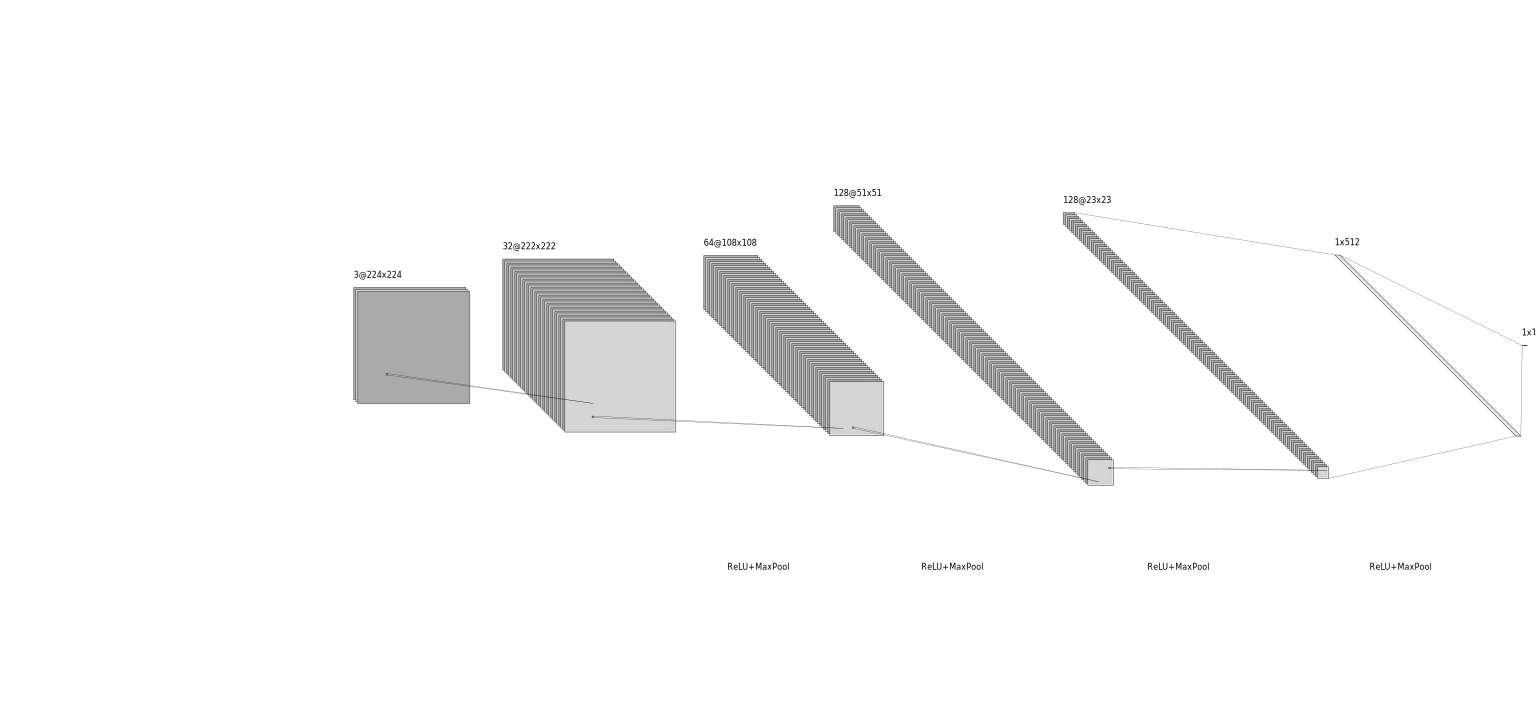
\includegraphics[width=\textwidth]{nn.png}
	\caption{The architecture of the convolutional network used. Visualization generated using \cite{nn-svg}.}
	\label{fig:architecture}
\end{figure}

Our input image has a dimension of $224 \times 224 \times 3$. The first layer is a 2D convolutional layer with 32 filters and a kernel size of $3 \times 3$, followed by a ReLU activation, and then by a max pooling layer with a pool size of $3 \times 3$ and a stride of 2. This is succeeded by 3 more layers which repeat the same sequence, but with 64, 128, and 128 convolution filters, respectively. After the last convolutional layer, a dropout layer with a factor of 0.5 is employed. This randomly sets a fraction of the previous layer's weights to zero---in this case, half of the weights---to prevent overfitting. This is followed by a 512-unit fully-connected layer, activated by ReLU. The output layer is a lone fully-connected unit which is activated by a sigmoid. All layers are initialized with a random Gaussian distribution of zero mean and unit standard deviation, and all biases are initialized to zero. Because our output has only one node but we expect it return a binary value, we select our loss function to be the binary cross entropy, defined as

\begin{equation}\label{eq:loss}
	H = -\frac{1}{N} \sum_{i=1}^N y_i \log[p(y_i)] + (1 - y_i) \log[1 - p(y_i)]
\end{equation}

\noindent where $y_i$ is the label, and $p(y_i)$ is the predicted probability of an image of having label $y_i$ for all $N$ images \cite{godoy}. For the optimizer, we use stochastic gradient descent (SGD) with learning rate $\eta = 0.01$, momentum $\mu = 0.9$, and a decay of $5 \times 10^{-4}$. We also use a learning rate scheduler, which reduces the learning rate by a factor of 10 if the validation loss does not improve over 5 epochs. Lastly, we also utilize a checkpointer, which saves a snapshot of the model weights if the validation loss decreases after an epoch. While monitoring the loss and accuracy, we now train the network until the validation loss drops below 0.1 or when the validation loss starts to diverge from the training loss.

\section{Results and Discussion}
Figure \ref{fig:loss-curves} shows the loss and accuracy curves after training the network. At epoch 13, the validation loss is minimum, and starts to diverge from the training loss afterwards. Training was manually stopped at epoch 29 after observing no further improvement in validation loss. We restored the best weights which were obtained at epoch 13, which had a validation loss and accuracy of $0.33$ and $87.00\%$, respectively. Overall training took around 80 minutes.

\begin{figure}[htb]
	\centering
	\includegraphics[width=\textwidth]{loss-acc.png}
	\caption{Loss and accuracy curves for the training and validation sets.}
	\label{fig:loss-curves}
\end{figure}

\noindent Feeding the test images in the network yields a loss of $0.15$ and an excellent $94.95\%$ accuracy. Sample predictions are shown in Fig. \ref{fig:outputs}. Only one out of the 18 predictions is wrong. Upon observation we can see why the network may have been confused: due to the dark color of the cat.

For increasing the accuracy of the network, one may consider adding another dropout layer after the deep fully-connected layer, playing around with the convolutional layer parameters, and using a deeper network.

\begin{figure}[htb]
	\centering
	\includegraphics[width=0.7\textwidth]{outputs.png}
	\caption{Sample filenames and predictions of cat and dog images.}
	\label{fig:outputs}
\end{figure}


\begin{table}[!htb]
	\centering
	\caption{Self-evaluation.}
	\begin{tabular}{||r|c||}
		\hline
		Technical correctness & 5 \\ \hline
		Quality of presentation & 5 \\ \hline
		Initiative & 2 \\ \hline
		\textbf{TOTAL} & \textbf{12} \\ \hline
	\end{tabular}
	\label{tab:self-eval}
\end{table}

\bibliographystyle{spp-bst}
\bibliography{biblio}

\end{document}